% Tämä on fysiikan laboratoriotöiden selostuspohjapohja.
% Pohja ei kuitenkaan ole mikään virallinen ja oikea totuus, 
% eli muistakin pohjia voi käyttää. Tämän tarkoitus on ainoastaan 
% auttaa opiskelijoita LaTeXin alkuun.
%
% Pohjaa saa levittää ja muuttaa vapaasti. Pohjan muuttajan toivotaan 
% kuitenkin lisäävän tiedot muutoksesta ja sen ajankohdasta tämän 
% kommenttiosuuden loppuun.  
%
% Pikainen käyttöohje:
% Päivita kansilehden tiedot
% Kirjoita selostuksesi
% ATK-keskuksessa käännät koodin seuraavilla komennoilla:
% use latex
% latex selkkari.tex
% 
% Esikatsele:
% xdvi selkkari
%
% Possuksi (tiedostonimeksi selostus.ps):
% dvips -o selostus.ps selkkari
%
% Toivottavasti tämä pohja auttaa alkuun
%
% Jukka Katainen, 6.2.2004
%
\documentclass[a4paper,11pt]{article}

\frenchspacing
\usepackage[finnish]{babel}
\usepackage[utf8]{inputenc}
\usepackage{graphicx}
\usepackage[T1]{fontenc}
\usepackage{float}
\usepackage{gensymb}

\begin{document}

%Tästä alkaa selkkarin kansilehti. Vaihda tilalle tarvittavat tiedot.
\begin{titlepage}
\pagestyle{empty}
\begin{center}

\vspace*{3cm}
\noindent\LARGE{\textbf{Työ 
%
%*******************************************************
%Työn numero:
14
%*******************************************************
%
\\
%
%*******************************************************
%Työn nimi:
Lämmönjohtavuus
%*******************************************************
%
}}\\
\vspace*{2cm}
Työvuoro \LARGE{\textbf{
%
%*******************************************************
%Työvuoro:
51
%*******************************************************
%
}} pari \LARGE{\textbf{
%
%*******************************************************
%Parin numero:
4
%*******************************************************
}}\\
\vspace*{1cm}
\large{
\begin{tabular}{l l}
%
%*******************************************************
%Parin opiskelijat ja opiskelijanumerot:
Juho Salmii & 80391C\\
Jukka Kemppainen & \\
%*******************************************************
%
\end{tabular}

\vspace*{1cm}
Selostuksen laati \emph{
%
%*******************************************************
% Selostuksen tekijä:
Juho Salmi
%*******************************************************
%
} \\
\vspace*{1cm}
\begin{tabular}{l l}
Mittaukset suoritettu & \textbf{
%
%*******************************************************
% Mittaukset suoritettu
25.11.2013
%*******************************************************
%
}\\
Selostus palautettu & \textbf{
%
%*******************************************************
% Selostus palautettu
2.12.2013
%*******************************************************
%
}\\
\end{tabular}
}
\end{center}
\end{titlepage}
%kansilehti loppuu tähän

%Varsinainan selkkari alkaa
\section{Johdanto}

Lämpöenergia on kineettistä energiaa hiukkastasolla. Lämmönjohtuminen tapahtuu, kun energia siirty hiukkaselta toiselle. Johtumista tapahtuu myös vapaasti hilassa liikkuvien elektronien diffuusion välityksellä. Eri aineilla on erilainen lämmönjohtavuus. Tässä työssä tutkitaan lämmönjohtavuutta erilaisissa materiaaleissa. \cite{wiki:thermal}

\section{Laitteisto ja menetelmät}

Työssä käytetään kuvassa \ref{laitteisto} esitettyä laitteistoa. Höyrygeneraattorilla tuotetaan 100\degree C vesihöyryä, josta se johdetaan höyrykammioon. Höyrykammion päälle asetetaan levy, jonka lämmönjohtavuuden ominaisuuksia tutkitaan. Levyn päälle asetetaan jääpala, jonka sulamisesta päätellään levyn lämmönjohtavuus. Jääpalan pinta on 0\degree C, joten lämpötilaero levyn puolien välillä on 100K. Tässä työssä tehdään mittaukset polykarbonaattilevylle sekä kahdelle lasilevylle. 

\begin{figure}[H]
\centering 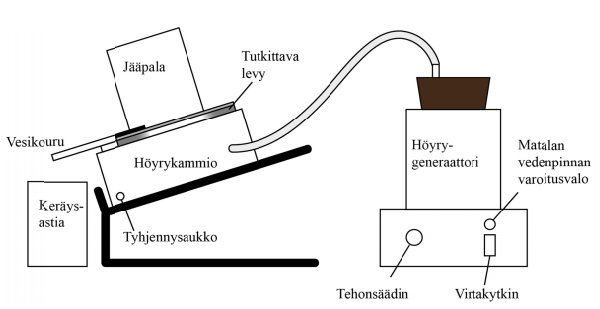
\includegraphics[width=0.8\textwidth]{laitteisto}
\caption{Työssä käytetty laitteisto. \label{laitteisto}}
\end{figure}

Lämpövirtaus on kääntäen verrannollinen lämpöä eristävän kerroksen paksuuteen

\begin{equation}
  \frac{\Delta Q}{\Delta t} = k A \frac{T_1 - T_2}{l} ,
\end{equation}

missä $\Delta Q$ on kerroksen läpi siirtynyt lämpömäärä ja, A pinta-ala $T_1 - T_2$ lämpötilaero, $l$ paksuus ja $k$ lämmönjohtavuuskerroin. 

Useampaa päällekkäisen kerroksen tapauksessa lasketaan niiden yhteenlasketut ominaisuudet seuraavasti: 

\begin{equation}
  \Delta T_{tot} = \sum_{i=1}^N (T_i - T_{i-1})
\end{equation}

\begin{equation}
  l_{tot} = \sum_{i=1}^N l_i
\end{equation}

\begin{equation}
  \frac{l_{tot}}{k_{tot}} = \sum_{i=1}^N \frac{l_i}{k_i}
\end{equation}

\begin{equation}
  \frac{\Delta Q}{\Delta t} = k_{tot} A \frac{\Delta T_{tot}}{l_{tot}} ,
\end{equation}

\section{Tulokset}

Mitataan alfalähteen säteilyn pulssitaajuus 5 mm etäisyydeltä vaimentamattomana sekä mylarkalvon kanssa. 
\begin{table}[H]
\begin{center}
\caption{Alfalähteen aiheuttama pulssitaajuus 5mm etäisyydeltä}
\begin{tabular}{ | r | l | }
  \hline 
  vaimentumaton & $4000 \pm 200 Bq$ \\ \hline
  mylarkalvon kanssa & $0,25 \pm 0,25 Bq$ \\ \hline
\end{tabular}
\end{center}
\end{table}

Mitataan alfasäteilyn kantama ilmassa siirtämällä alfalähdettä kauemmas detektorista. Saadaan, että $23 \pm 1 mm$ etäisyydellä detektori ei havaitse kuin satunnaisia hajoamisia, joten etäisyys voidaan katsoa alfasäteilyn kantamaksi. 

Mitataan beetalähteen säteilyn pulssitaajuus 5mm etäisyydeltä vaimentamattomana, mylarkalvon ja pleksilevyn kanssa.
\begin{table}[H]
\begin{center}
\caption{Beetalähteen aiheuttama pulssitaajuus 5mm etäisyydeltä}
\begin{tabular}{ | r | l | }
  \hline
  vaimentumaton & $350 \pm 50 Bq$ \\ \hline
  mylarkalvon kanssa & $350 \pm 50 Bq$ \\ \hline
  pleksilevyn kanssa & $125 \pm 25 Bq$ \\ \hline
\end{tabular}
\end{center}
\end{table}
   
Mitataan beetasäteilyn vaimenemista siirtämällä beetalähde niin kauas detektorista kuin mittalaitteella on mahdollista. Saadaan maksimietäisyydellä $83 \pm 0,5 mm$ pulssitaajuudeksi $75 \pm 25 Bq$. 

Kaavasta \ref{annosnopeus} saadaan laskettua alfasäteilyn mylarkalvoon aiheuttama annosnopeus: $0,02 J/kg \cdot s$

Beetasäteilyn pleksilevyyn aiheuttaman ekvivalenttiannoksen annosnopeus: $0,12 \mu J / kg \cdot s$


\subsection{Gammasäteily}
\label{tulokset:gamma}

Mitataan gammalähteen pulssien lukumäärää eri etäisyyksiltä tasavälisesti $1/r^2$ suhteen kymmenen sekunnin ajan. Etäisyyden virheeksi arvioidaan $\pm 0,1 cm$ ja pulssimäärän virheeksi $\sqrt{n}$.

\begin{table}[H]
\begin{center}
\caption{Gammalähteestä mitattujen pulssien määrä eri etäisyyksiltä 10 s aikana}
\begin{tabular}{ | r | l | }
  \hline
Etäisyys (cm) & Havaitut pulssit (kpl) \\ \hline
5.0 & 2704 \\ \hline
5.3 & 2474 \\ \hline
5.7 & 2061 \\ \hline
6.1 & 1830 \\ \hline
6.7 & 1552 \\ \hline
7.4 & 1320 \\ \hline
8.5 & 1005 \\ \hline
10.3 & 743 \\ \hline
14.1 & 523 \\ \hline
40.0 & 319 \\ \hline
\end{tabular}
\end{center}
\end{table}


Kuvaajasta saadaan kulmakertoimeksi $k = \frac{\Delta{n}}{\Delta \frac{1}{r^2}} = 62 000 cm^2$. Sen avulla voidaan ratkaista kaavasta \ref{pulssitaajuus} aktiivisuus, kun $\dot{n} = \frac{\Delta n}{\Delta t}$ 

\begin{equation}
  A = \frac{\Delta n}{\Delta \frac{1}{r^2}} \frac{4 \pi }{\epsilon \cdot n_A \cdot a_d \Delta t} = 0,021 MBq ,
\end{equation}

Tarkistetaan saatu vastaus puoliintumisajan avulla. Lähteen aktiivisuus vuonna 1987 oli 0,62 MBq, joten sen aktiivisuus on ehtinyt puoliintua 4,93 kertaa. 

\begin{equation}
  A = 0,62 {MBq} \cdot \frac{1}{2^{4,93}} = 0,020 {MBq} ,
\end{equation}

Mitataan gammalähteen pulssien lukumäärä 20 cm etäisyydeltä 100 s ajan eri määrällä lyijylevyistä valmistettuja absorptiolevyjä. 

\begin{table}[H]
\begin{center}
\caption{Gammalähteestä mitattujen pulssien määrä 20 cm etäisyydeltä 100 s aikana eri lyijykerroksen paksuuksilla}
\begin{tabular}{ | r | l | }
  \hline
Lyijyn määrä (mm) & Havaitut pulssit (kpl) \\ \hline
0 & 4000 \\ \hline
2 & 3797 \\ \hline
4 & 3801 \\ \hline
6 & 3554 \\ \hline
8 & 3535 \\ \hline
12 & 3330 \\ \hline
16 & 3315 \\ \hline
20 & 3003 \\ \hline
28 & 2809 \\ \hline
36 & 2655 \\ \hline
50 & 2576 \\ \hline
80 & 2193 \\ \hline

\end{tabular}
\end{center}
\end{table}

Kuvaajan perusteella voidaan päätellä, että intensiteetin puoliintumispaksuus on n. 25 mm. 10 \%:iin intensiteetti laskee jossakin 60--70 mm tienoilla. 

Mitataan dosimetrillä säteilyannosta työskentelypaikalta lyijytiilien kanssa, ilman lyijytiiliä sekä 5 cm päässä gammalähteestä. 

\begin{table}[H]
\begin{center}
\caption{Dosimetrin lukemat 5 cm etäisyydeltä}
\begin{tabular}{ | r | l | }
  \hline
  lyijytiilien kanssa & $0,18 \pm 0,01 \mu Sv /h$ \\ \hline
  ilman lyijytiiliä & $0,18 \pm 0,01 \mu Sv /h$ \\ \hline
  5 cm päässä lähteestä & $0,50 \pm 0,05 \mu Sv /h$ \\ \hline
\end{tabular}
\end{center}
\end{table}

Dosimetrimittauksen perusteella säteilylähde ei juurikaan kasvata annosnopeutta taustasäteilyyn verrattuna. 

\section{Yhteenveto ja pohdinnat}

Havaitaan, että alfasäteily pysähtyy ohueenkin väliaineeseen, siinä missä beetasäteily läpäisee vähän paksummankin väliaineen. Gammasäteily puolestaa läpäisee jopa paksumman lyijykerroksen. Samalla tavalla käyttäytyvät myös säteilytyyppien kantamat. Alfasäteilyltä on helppo suojautua, mutta siitä saa nopeasti suuren ekvivalenssiannoksen. 

Mittauksia tehdessä, olivat tutkimuksen tekijät pääsääntöisesti suojattu säteilyltä, eikä lähelläkään säteilylähdettä ollut vaarallisia annosnopeuksia. Ainoa elin, joka joutui lähelle säteilylähdettä oli käsi, ja sen efektiiviset painokertoimet ovat pieniä. 


%Kirjallisuuviitteet
\begin{thebibliography}{99}
% Kirjallisuus viitteet tähän tapaan:
%\item{R.W. Robinnet, Quantum Mechanics, Oxford University Press, 1997}

\bibitem{ohje} Harjoitustyöohje: Työ 14 Lämmönjohtavuus, http://physics.aalto.fi/pub/kurssit/Tfy-3.15xx/materiaali/14.pdf [Viitattu 18.11.2013]
\bibitem{wiki:thermal} Wikipedia-artikkeli lämmönjohtavuudesta, http://en.wikipedia.org/wiki/Thermal\_conduction [Viitattu 2.12.2013]

\end{thebibliography}

%liitteet numeroituna
\section*{Liitteet}
\begin{enumerate}
%Liitteet tähän tapaan
\item{Mittauspöytäkirja}\label{mittaus}

\end{enumerate}

\end{document}
